\subsection{Application}
The Application is composed of two different sub-components (Figure
\ref{fig:sd-app-init}):

\begin{itemize}
  \item \textbf{Application Logic Layer}: handles the application logic
    (slightly abusing the notation, we will often refer to it simply as
    \textit{Application Layer});
  \item \textbf{Interface Layer (IL)}: provides the remote services to Application
    Layer by acting as an interface towards the underlying middleware layer.
\end{itemize}

In the next sections we will use the following terms to describe the state of a
software layer or a package:
\begin{itemize}
	\item \verb|inactive| - not even created;
	\item \verb|ready| - initialized with all the needed resources. Not yet
	allowed to execute;
	\item \verb|active| - executing;
	\item \verb|stopped| - not executing. It is waiting to terminate.
\end{itemize}

\subsubsection{Application Layer}

The main packages have been named according to Table \ref{tab:entity_type}.
\subsubsection{Interface Layer}

Figure \ref{fig:impl-il-arch} provides an high level view of
the Interface Layer (IL) components.

\begin{figure}[H]
  \centering
  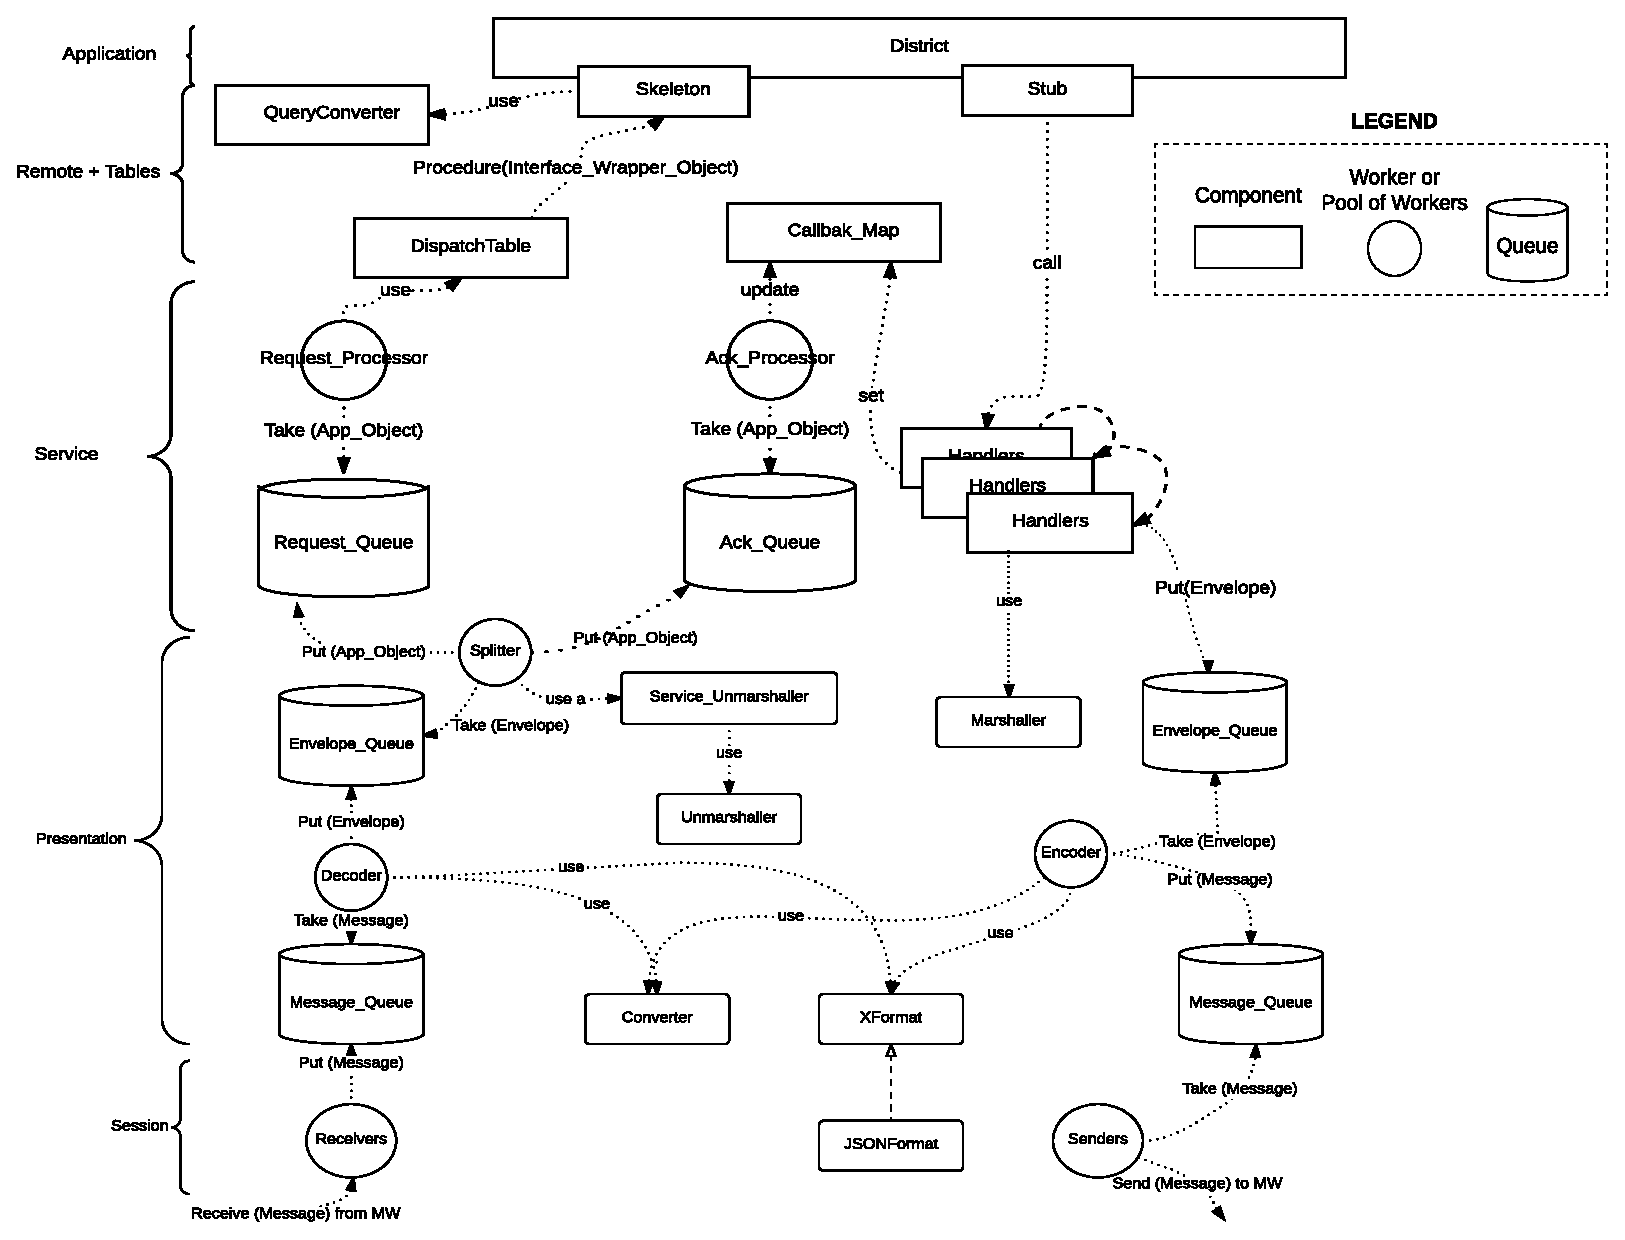
\includegraphics[width=\columnwidth]{images/solution/il.eps}
  \caption{Interface Layer architecture}
  \label{fig:impl-il-arch}
\end{figure}

IL enables the Application Layer to communicate with other applications
transparently without knowing if they are local or remote. We encapsulate the
application data as message payload while
different sublayers of IL manipulate different fields of the
message header.
This layered approach has been inspired by the TCP/IP and ISO/OSI models, in
which the layers communicate in two directions:
\begin{itemize}
	\item horizontally - manipulating the same fields of the header;
	\item vertically  - passing the packet to the next
layer, which is charged with different responsibilities.
\end{itemize}
Also, IL is completely asynchronous because each of its sublayers has its own
thread pool. Furthermore, each thread pool is controlled by a master thread which
runs in an event loop consuming messages from its own incoming
queue. For example, the receiver can handle potentially multiple concurrent
requests by delegating each one of them to its worker threads.
After a worker has
completed the assigned task it is pushed back on the receiver's local stack,
ready to be reused.


In the following we list the sublayers which compose IL in
bottom up order:

\begin{itemize}
  \item \textit{Session Layer} --
  handles remote connections through TCP sockets;
  \item \textit{Presentation Layer} --
  handles messages formatting and conversions;
  \item \textit{Service Layer} --
  converts remote requests into procedure calls
  by leveraging a skeleton object.
  Also, it offers the specular service through a stub object plus a pipeline
  of handlers. For each request, the former compose a specific pipeline
  of handlers transparently to the Application Layer.
  The handlers are used to incrementally construct the message by adding
  header fields, wrapping the data into a payload field and finally putting
  the message in the first queue which goes downwards (towards the middleware).
  \item \textit{Remote Layer + Tables} --
  It contains the tables used
  to dispatch the remote calls and the callback map of pending requests.
  A pending request is a synchronous requests which may trigger one of
  the following behaviors:
  \begin{itemize}
  	\item retransmission on timeout;
  	\item a local retry on failure - retry on the local district with
  	the next action which could be a repetition of the last executed action;
  	\item a local clean up on success - remove the retained data from the local
  	district. The message has been successfully sent.
  \end{itemize}
  With pending request we are not reinventing a weakened version
  of TCP retransmission timers as it might seem.
  Indeed, we have concretely faced network connection errors during
  the communication
  with the middleware layer. This was caused by occasional failures or network
  problems subsequently fixed by the system itself
  (i.e., the docker swarm node).
  However,
  we preferred to give the responsibility of these synchronous messages to IL
  for two reasons:
  \begin{itemize}
  	\item it is the layer which has the highest probability of not losing them.
  	Indeed, the communication with the Application Layer happens through
  	local procedure
  	calls. Also, the TCP communication with the middleware layer could lead to
  	lose messages;
  	\item the data wrapped in the messages are important for the
  	application which can not afford to lose them. Indeed, a lost message
    could mean a missing pedestrian in the system. Thus, a failure
  	or a timeout has to trigger a reaction as soon as possible because
  	the latency introduced in the communication can lead to a significant
  	time drift for the end user (e.g., a set of travellers blocked with
  	apparently no reason). This could undermine the principle of viewing the
  	whole distributed system as one single unit.
  \end{itemize}
\end{itemize}
\subsubsubsection{Bootstrap}
In order to neatly start the application layer, we have to consider the
dependencies among the entity types exposed in \ref{fig:sd-entity-types-deps}.
Moreover we have to take into account that this layer can not decide by itself
when it is time to start, because this is ruled by the middleware.
The bootstrap process, which mimics the UNIX init (i.e. initd and runlevels)
is divided in two ordered parts:
\begin{enumerate}
	\item \textit{init} - initialize all the sub-layers of each macro layer
	following a bottom up approach (from \verb|interface_layer.session| to \verb|application.scheduling|). The order is inferred by the fact that the upper
	layers need the services provided by the underlying layers to work
	correctly. This event is automatically triggered when the node is created.
	\item \textit{start} - the first tick forwarded from the middleware to the
	application layer through the interface\_layer. As stated, this event is
	exclusively triggered by the middleware.
\end{enumerate}
Also, the application node is divided in two macro layers:
\begin{itemize}
	\item \textit{Interface layer} - provides network services to
	application layer (e.g. session, marshalling, etc.) and acts as an interface
	for the application towards the underlying layers (i.e. middleware);
	\item \textit{Application layer} - implements the city logic
	(e.g. movements of entities in the streets).
\end{itemize}
Each application node contains the \textit{Init} process,
which is the parent of all the application processes.
Init instantiates the resources of each layer triggering the switch of the
interface\_layer state from \verb|inactive| to \verb|ready|.
Also, each sub-layer of interface\_layer has its own pool of LWP.
The application layer initialization completes in the following order:
\begin{enumerate}
	\item \textit{Active} - the entities which moves in the city (e.g. pedestrians);
	\item \textit{Reactive} - the infrastructure of the city (e.g. district);
	\item \textit{Scheduling} - the sub-layer which handles the execution order and
	synchronization signals of each event of the application layer.
\end{enumerate}
Note that the \textit{Passive} entities have no particular dependency. Since
they are stateless and they logically belong to \textit{reactive} entities
(e.g. road signs belong to roads), they will be instantiated along with them.
When the scheduling sub-layer completes its initialization, init signals
the application layer completion to each sub-layer of interface\_layer in the
following order:
\begin{enumerate}
	\item \textit{service} - provides activators and pipelines services to
	application layer;
	\item \textit{presentation} - provides data conversion services;
	\item \textit{session} - provides network connection services
	(e.g. sender, receiver).
\end{enumerate}
This signal triggers the switch of each sub-layer of interface\_layer state from
\verb|ready| to \verb|active|.
The activation order is extremely important to
proactively avoid the lost of messages between remote nodes. Indeed, at this
stage, the application layer is not able to generate or receive messages
because the start message has not been sent by the middleware.
The service and
the presentation layer are activated before the session layer; the latter
exposes a remote communication channel (a connection to a TCP socket).
Moreover, the interface layer follows the nginx concurrency model using a
pool of workers and an event loop to handle multiple concurrent requests
with different queues for different requests (e.g. blocking and asynchronous).
Finally, the application is ready to communicate because each of its layers
has been activated.
% TODO: Review this things

\begin{figure}[H]
  \centering
  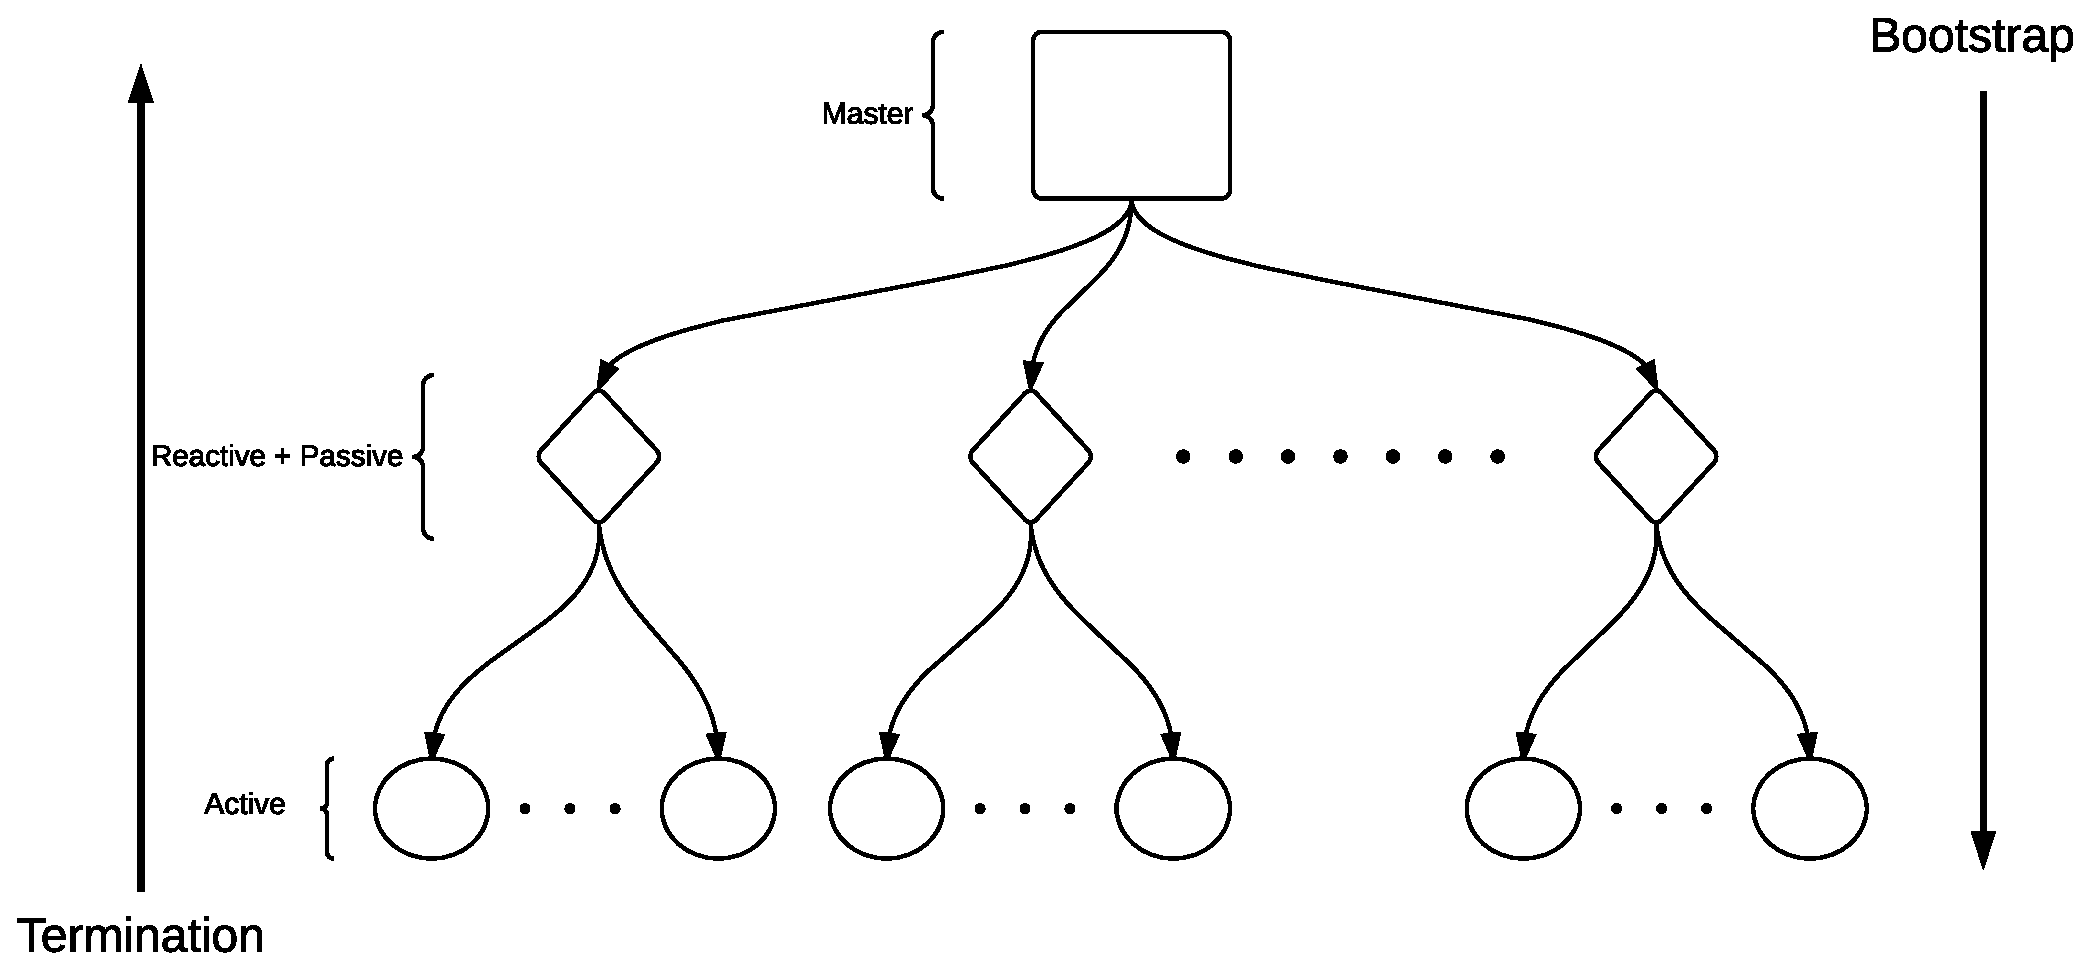
\includegraphics[width=\columnwidth]{images/solution/app_proc_tree.eps}
  \caption{Application process tree}
  \label{fig:app-proc-tree}
\end{figure}

At the end of the bootstrap, the \textit{Init} process has to notify the
middleware layer of the successful completion and the middleware has forwarded
the start message to the application. A crash of the
\textit{Init} process, occurring before the end of the bootstrap,
is signaled to the middleware layer, by the expiration of a timeout from the
middleware side.
Note that this model works also for a bootstrap which is executed starting
from a snapshot of the system, with the only difference consisting in divergent
values of the configuration file. Indeed, we have to use a set of
configurations, which is going to be different for each city.
\subsubsection{Termination}

When describing the shutdown of the whole system, we assumed the application
terminates gracefully.
In this section we show the algorithm we designed to achieve this goal.

As we can see from figure \ref{fig:termination-app}, the termination follows the
opposite order of the bootstrap.

\begin{figure}[H]
  \centering
  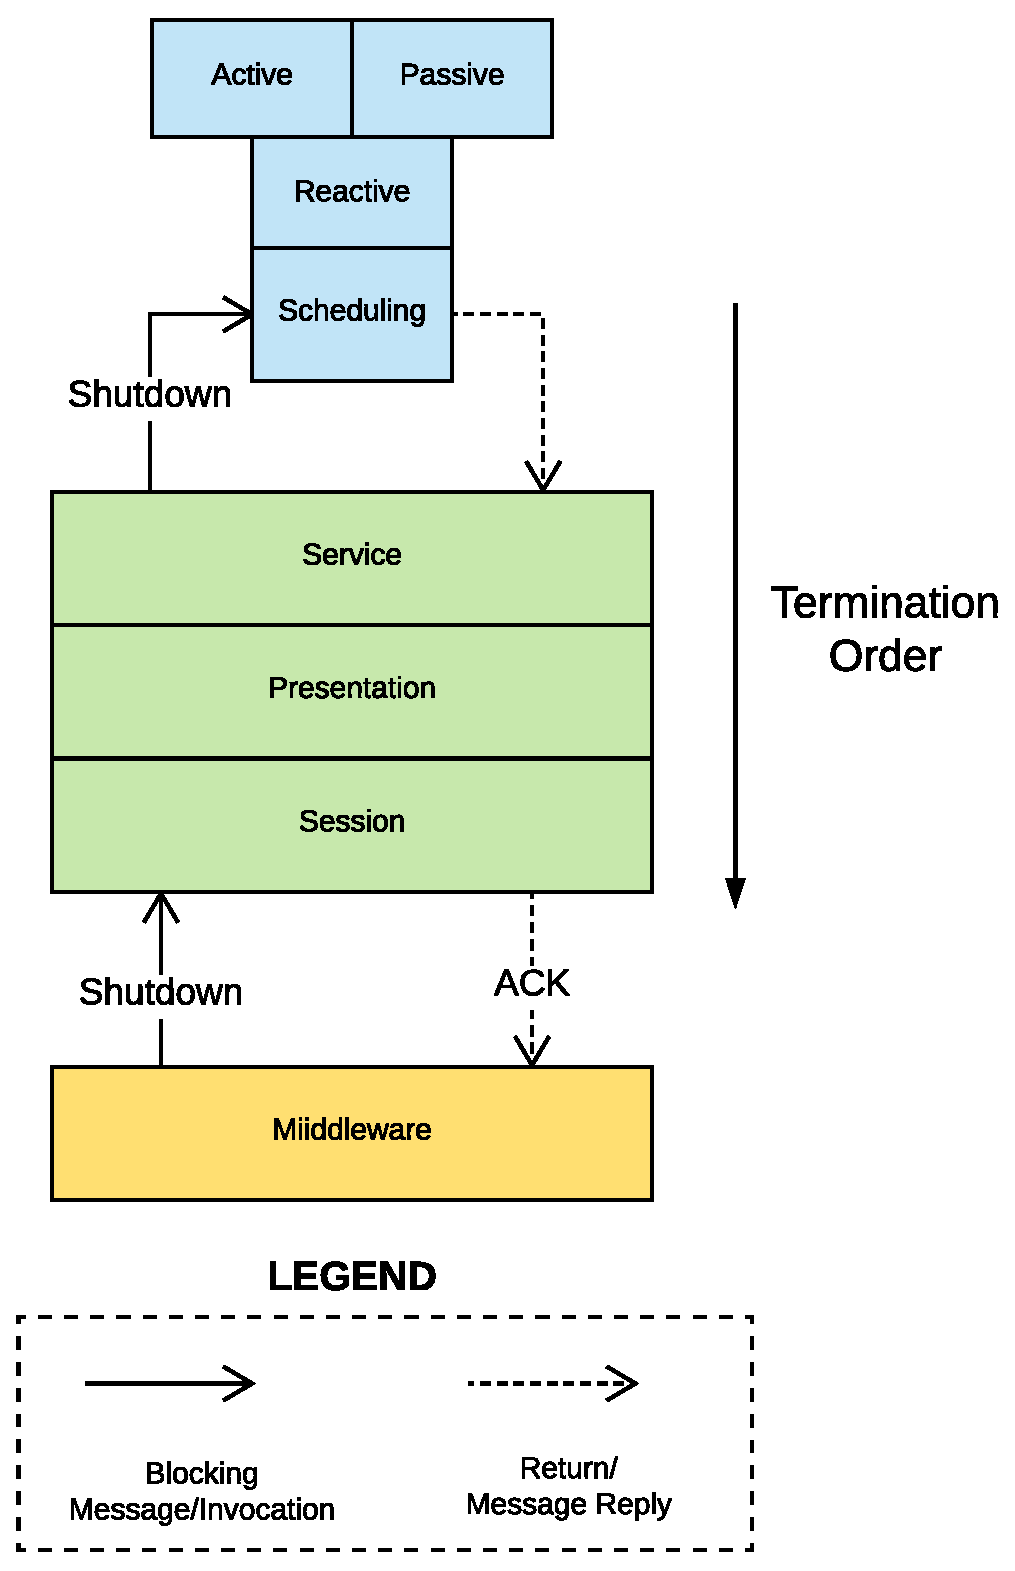
\includegraphics[scale=0.4,keepaspectratio]
    {images/solution/termination-app.eps}
  \caption{Application Termination}
  \label{fig:termination-app}
\end{figure}

%TODO: Review termination process
\begin{enumerate}
  \item The middleware sends a \verb|shutdown| message to IL;
  \item The upwards components\footnote{these components carry the messages
  from middleware to the application layer} of the sublayers of IL terminates
  themselves when they
  read the shutdown request in the header. This is achieved by a transition
  from \verb|active| to \verb|stopped| state, which enables the master
  of each event loop to wait for all its workers to complete. Then the master
  puts the shutdown notification in the queue of the next IL component;
  \item The shutdown message is forwarded upwards until it reaches the Scheduling
  component. Then the scheduler notifies its workers. The workers change their
  state to \verb|stopped| and wait on a barrier until all the other workers have
  completed their execution. \\
  At this stage, we have the guarantee that no worker is running at
  the Application Layer level. Indeed, all the Application Layer
  entities are inerts because their engine (i.e., the scheduler) has been
  turned off;
  \item The previous point implies that we can safely terminate
  also the downwards components of the IL subsytem. Indeed, no message
  will be sent if the scheduler is not running. Thus, as last message
  an acknowledgment to the shutdown request
  originally sent by the middleware is packed
  by the stub component and sent downwards through the IL forwarding pipeline;
  \item All the downwards components of IL behaves exactly as the upwards one;
  \item The sender component forwards the acknowledgment message
  to the middleware.
\end{enumerate}


We implement also a dump method, to enable each stateful entity to save its
state before terminating. However we have not
been able to test it successfully in the distributed environment. Thus, we
kept it in the source code but we did not use it in production.



Similarly to the bootstrap phase, the middleware expects to receive the
\verb|shutdown| ack message within a certain amount of time.
In order to do so, when sending the message, the middleware starts a timeout.
Wherefore if it expires before receiving a response message,
it retransmit again the \verb|shutdown| request towards the application.

\subsubsubsection{Interaction between entities}

The application contains several interactions among entities that have to be
specified in order to understand well how to approach different problems.

\paragraph{Entering a road} Moving entities enter a road by entering a stretch
that is located at the beginning of the road and that is treadable by their
specific entity type.

\paragraph{Entering a road stretch} Moving entities who want to enter a new
road stretch can do it whenever there is room for them in that stretch. In
particular, a roadway stretch can be trod for at most one vehicle at the same
time.

\paragraph{Zebra crossings} Vehicles which want to enter a road stretch that
has zebra crossings painted on it has to wait for pedestrians or bikes to free
all stretches of that particular crossing.

\paragraph{Changing roadway lane} A vehicle that is on the i-th road stretch
which wants to change lane has to wait until the (i+1)-th stretch in the
wanted direction is free.

\paragraph{Crossroads} Every road that is connected to a crossroads is marked
with a cardinal point (N/E/W/S). The crossroads holds all the logic necessary
for vehicles to follow the yield rules we described in
\ref{sec:pa-domain-problems}.

There could be a situation in which there is a standstill, for example when
four cars want all to go straight in a four-way crossroads. In this case, the
crossroads will make a car yield the right-of-way to another one.

Pedestrians can only walk on the corner of the crossroads, thus passing to the
adjacent piece of road (e.g. a pedestrian that is coming from the ``southern''
side of the western road can only enter the southern street on the ``western''
side).

\paragraph{Entering a building} When a moving entity is in the stretch where
there is the entrance of a building, then it may enter the building.

If the moving entity is a vehicle, it has to wait for all other entities who
are in the intermediate stretches to move away.

\paragraph{Exiting a building} When a moving entity is exiting a building, it
has to check whether there is room for her to move out.

If the entity is a vehicle, it has to yield the right-of-way to upcoming
vehicles and to wait that eventual sidewalks or bicycle path stretches in front
of the building are free too.

\paragraph{Choosing to use a vehicle} An entity $e$ who wants to leave a
building $b_e$ to a destination $d_e$ may randomly decide not to travel by
foot. She can leave only if:

\begin{itemize}
  \item the path from $b_e$ to $d_e$ does not include any destination of other
    people who are leaving from $b$ and viceversa. Otherwise, they would share
    the vehicle if there is enough room;
  \item there is an available vehicle in $b_e$; and
  \item the capacity of the destination building $d_e$ is greater than the sum
    of all vehicles in it and the ones which are arriving to that building.
\end{itemize}

If all of these conditions are met, then:
\begin{itemize}
  \item the entity may exit the building and travel using a vehicle; and
  \item $d_e$ now ``books'' a place for the vehicle driven by $e$.
\end{itemize}

\paragraph{Waiting for a bus} A pedestrian may randomly decide to wait for a
bus if she is on a bus stop stretch.

Firstly, she checks whether the buses that stops at that stretch match (even
partially) her path. If at least one of them does, then she wait for a limited
amount of time for a bus to arrive.

If this timeout expires, then she continues travelling by foot to the next
stretch.

\paragraph{Boarding a bus} When a bus arrives at a bus stop, then a waiting
entity will board it only if:

\begin{itemize}
  \item there is enough room for her; and
  \item this bus shortens the expected route for her.
\end{itemize}

\paragraph{Getting off a bus} A person $p$ will get off a bus when it reaches
the last stop $s$ such that $s$ belongs to the route of $p$.

\paragraph{Respecting street code} Roads and crossroads will contain all the
necessary logic to make moving entities follow the street rules.

\paragraph{Performing an overtaking} This action is possible only when a
vehicle is able to change lane. It might be triggered by a timeout which
expires when it is waiting too much for entering the next straightaway stretch.

When a vehicle tries to overtake another one, it will always try to return to
the lane where it started the operation before entering the last stretch.
% look for "manovra" translation

% \paragraph{Uber} % Is it a TODO?


% Detail design
\subsubsection{Detailed Design}

\subsubsection{Detailed Design}
\subsubsubsection{Active Entity}
\subsubsubsubsection{Moving entity}
\begin{figure}[h]
\centering
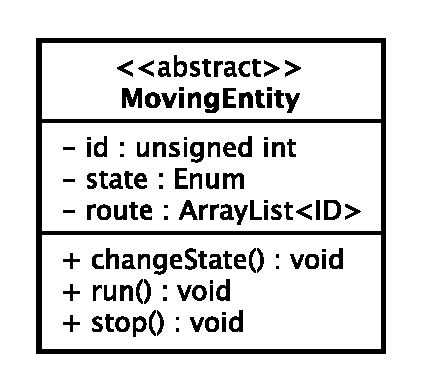
\includegraphics[scale=0.6,keepaspectratio]{images/solution/moving_entity.eps}
\caption{App::Active::MovingEntity}
\label{fig:sd-app-movingentity}
\end{figure}
\FloatBarrier
\begin{itemize}
  \item \textbf{Description} \\
    It represents an entity that moves through the city, consuming its 
route at each stretch treaded.
  \item \textbf{Attribute}
  \begin{itemize}
    \item \texttt{- id: Unsigned Int} \\
A unique identifier, useful to keep track of each entity.
    \item \texttt{- state: Enum} \\
The possible states of the entity \{ running, stopped \}.
    \item \texttt{- route: ArrayList<UrbanEntity>} \\
The route of urban entities that the entity has to tread.
    \item \texttt{- maxSpeed: Unsigned Int} \\
The maximum possible speed for the entity.
  \end{itemize}
  \item \textbf{Operation}
  \begin{itemize}
    \item \texttt{- changeState(state: Enum)} \\
Change the entity state. This method is used internally by public methods to 
change the entity behaviour.
    \item \texttt{- setSpeedLimit(speed: Unsigned Int)} \\
Updates the maximum speed of the entity.
    \item  \texttt{+ MovingEntity(route: ArrayList<UrbanEntity>)} \\
Creates a moving entity setting its route.
    \item  \texttt{+ run()} \\
Activates the entity which sets its state to \textit{running} and 
starts consuming its route.
    \item  \texttt{+ stop()} \\
Stops the entity which sets its state to \textit{stopped}.
   \item  \texttt{+ getMaxSpeed() : Unsigned Int} \\
Returns the maximum speed of the entity.
     \item  \texttt{+ getId() : Unsigned Int} \\
Returns the id of the entity. 
    \item  \texttt{+ notify(house: House) : ArrayList<Pedestrian>} \\
Decide if it want to rest in the house according to its route: in this case
returns a list of pedestrian which wants to stay in the house, otherwise returns
an empty list.
    \item  \texttt{+ update(roadsign: RoadSign) : boolean} \\
Check the road sign concrete type and then behaves according to it (i.e. if the
road sign is a speed limit it updates its maxSpeed using this.setSpeedLimit(roadsign.getLimit())). Returns true if completed correctly/action accepted, false otherwise.
  \end{itemize}
\end{itemize}

\subsubsubsubsection{Vehicle}
\begin{figure}[h]
\centering
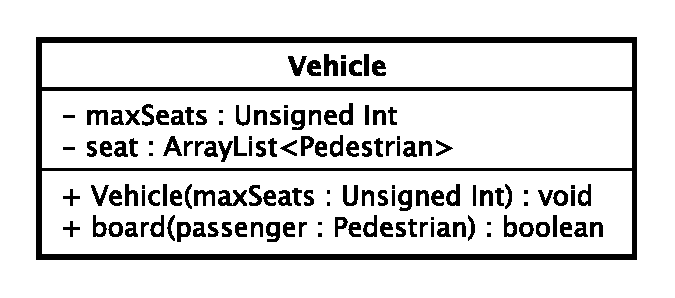
\includegraphics[scale=0.6,keepaspectratio]{images/solution/vehicle.eps}
\caption{App::Active::Vehicle}
\label{fig:sd-app-vehicle}
\end{figure}
\begin{itemize}
  \item \textbf{Description} \\
    It represents an entity that moves through the city carrying one or more
pedestrians.
  \item \textbf{Attribute}
  \begin{itemize}
    \item \texttt{- maxSeats: Unsigned Int} \\
The maximum number of seats in the vehicle.
    \item \texttt{- seat: ArrayList<Pedestrian>} \\
The list of passengers carried by the vehicle.
  \end{itemize}
  \item \textbf{Operation}
  \begin{itemize} 
    \item \texttt{+ Vehicle(maxSeats: Unsigned Int)} \\
Creates a vehicle specifying its maximum number of seats.
    \item \texttt{+ board(passenger: Pedestrian) : boolean} \\
If the vehicle is not full the pedestrian become a passenger and the method 
returns \textit{true}. Otherwise the access to the vehicle is not granted and 
the method returns false.
  \end{itemize}
\end{itemize}

\subsubsubsection{ReactiveEntity}
\subsubsubsection{PassiveEntity}

